%---------------------------------------------------------------
%	PACKAGES AND OTHER DOCUMENT CONFIGURATIONS
%--------------------------------------------------------------
\documentclass[paper=a4, french, 11pt]{scrartcl} 

\usepackage[utf8]{inputenc} 
\usepackage[T1]{fontenc} % Use 8-bit encoding that has 256 glyphs
\usepackage{fourier} 
\usepackage[francais]{babel} % English language/hyphenation
\usepackage{amsmath,amsfonts,amsthm} % Math packages
\usepackage{colortbl}
\usepackage{graphicx}
\usepackage{sectsty} % Allows customizing section commands
\usepackage{fancyhdr} % Custom headers and footers


\allsectionsfont{\centering \normalfont\scshape} 

\sectionfont{\normalfont\scshape}
\subsectionfont{\normalfont\scshape}
\subsubsectionfont{\normalfont\scshape}

\pagestyle{fancyplain} 
\fancyhead{} 
\fancyfoot[L]{} % Empty left footer
\fancyfoot[C]{} % Empty center footer
\fancyfoot[R]{\thepage} % Page numbering for right footer
\renewcommand{\headrulewidth}{0pt} % Remove header underlines
\renewcommand{\footrulewidth}{0pt} % Remove footer underlines

\setlength{\headheight}{13.6pt} % Customize the height of the header
\setlength\parindent{0pt} 

\definecolor{bg}{RGB}{235,235,235}
\definecolor{bk}{RGB}{135,135,135}
\newcommand{\class}[1]{\colorbox{bg}
{\textcolor{red}{\usefont{OT1}{cmtt}{m}{n}#1}}}
\newcommand{\cmd}[1]{\colorbox{bk}{\textcolor{white}
{\usefont{OT1}{cmtt}{m}{n}#1}}}
\newcommand{\horrule}[1]{\rule{\linewidth}{#1}}

%-----------------------------------------------------------
%	TITLE SECTION
%-----------------------------------------------------------

\title{	
\normalfont \normalsize 
\textsc{Projet INF582} \\ [25pt] 
\horrule{0.5pt} \\[0.5cm] % Thin top horizontal rule
\huge Text detection \\ % The assignment title
\horrule{2pt} \\[0.5cm] % Thick bottom horizontal rule
}

\author{Zhixing CAO, Yuesong SHEN} % Your name

\date{\normalsize\today} % Today's date or a custom date

\begin{document}

\setlength\parindent{12pt}
\maketitle % Print the title

\section{Introduction}
The development of smartphones and the growing demands in content-based image understanding has made the text detection a crucial topic in machine-human interaction. It has been shown that the performance of image retrieval depends critically on the performance of text detection and recognition. For example, two book covers with different titles but identical background prove to be considered virtually indistinguish without detecting and recognizing the text.

\subsection{Goal of project}
Early approach of text detection and recognition techniques such as OCR can be traced in early 1900s. Recent years, with the progress in the field of machine learning pattern recognition and text localisation techniques make new breakthroughs. With the study of some of those techniques, our project concern algorithms that can decode the text in images.

The approach of our project can be divided into two parts --- text detection and text recognition. The detection part detect potentiel texts in images and output pure text candidates and the recognition part translate the image of text candidates to digital texts that can be read by machines.

\subsection{Work breakdown}
The whole project is carried out by Zhixing CAO and Yuesong SHEN. Several works have been carried out independently during the project. Here is the overview of work breakdown.\
\begin{figure}
	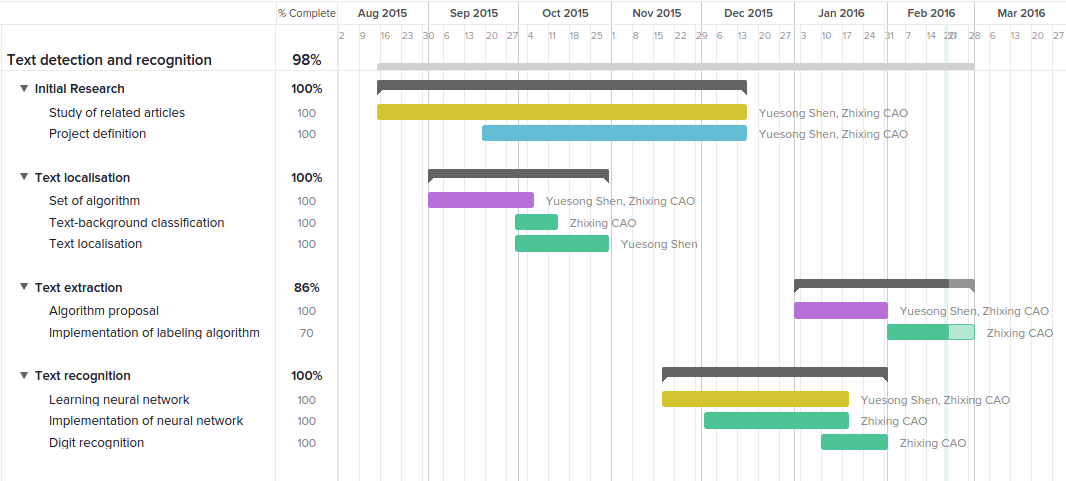
\includegraphics[width=0.7\paperwidth]{breakdowns.png}
\end{figure}
 
\section{State of the art}
\subsection{Text detection}
As an essential prerequiste for text recognization, text within images has to be robustly located. This is challenge task due to the variety of the text form, such as variations in languages, font and style, geometric and photometric distortions, partial occlusion, and lightening conditions. Text detection problem have been studied a lot in recent researches and numerous methods are reported in the literature.

All the methods used in recent research can be classified into two catagories: method based on texture and method based on connected componet.

Texture-based method views texts as a special texture that is distinguish from its background. Features are extracted over some special regions and a classifier is used to identify texts areas. Zhong and al have segmented caption text regions from background and used the intensity variation information. Ye and al have proposed a method using multiscale wavelet featires and a coarse-to-fine algorithm to locate text lines under different backgrounds.

Different with the texture-based method, the connected component based approach extrats regions from the image and selects text candidates using some geometric rules. In ICDAR 2005 text locating competition, the best result applies have used an adaptive binarization method to find connected components and forms text lines based on geometric properties. Recently Chen and al extract letter candidates by employing edge-enhanced Maximally Stable Extremal Regions and using geometric and stroke width information to exclude non-text objects. They have achieved an accuracy score of 95\%.

\subsection{Text recognition}
Converting text data from image and deciphering into digits is an important problem. Early physical photocell-based OCR implemented matrix matching by comparing an image to a stored glyph on a pixel-by-pixel based. Those algorithms involve mostly extensive processing on the image such as thinning, smoothing contour analysis etc. because the majority of previous works uses geometrial and topological features. In recent research community the dominant approach to this problem is based on machine learning techniques --- a general inductive process builds automatically a classifier by learning.

In the textbook \textit{Pattern Recognition and Machine Learning}, Bishop reflects recent developments in the field of pattern recognition and machine learning and shows potential usages of machine learning method in patter recognition. The early effort has been made around 1986s by Burr, Mehr\&Richfield to implement a neural networks in character recognition. Recently, with the development of paralel computation and the use of GPU, efficiant OCR system based on neural network is realized. 

\subsection{Our approach}
In this report, we show you our approach of the text detection problem by combined texture-based method and connected component based method and our text recognition algorithm using neural network. 

We adapte at first the method proposed by Liu and al to locate texts. This algorithm detects text candidate by applied classifier on contour pictures of the original image. Experimental results demonstrate that this approach is robust for font-size, font-color, background and languages, which can be used efficiently.

After locating the text, a connected component based method is used to extract word candidates. We find all components by using connected-component labeling algorithm. Then we use some geometric constraints and heuristic rules to merge them and extract letters and words candidates.  

Our approach for text recognition is based on using neural network to classify characters. With a training set of different kind of characters, the neural network is constructed in order to match an input character to a learned one. 

\section{Text detection}
\subsection{Detecton of contour}
\subsection{K-means classification}
\subsection{Text area identification}
\subsection{Connected components detection}
\subsection{detection of words}

\section{Text recognition}
\subsection{Neural network}
\subsection{Pattern Recognition}

\section{Conclusion}

\end{document}